\documentclass[a4paper,10.0pt,twoside]{npr}

\usepackage{multicol,graphicx,lastpage,footmisc,fancyhdr,paralist,
tabularx,array,booktabs,caption,multirow,upgreek,mathrsfs,gensymb,color}
\usepackage[fancyhdr,space,fntef,fontset=ubuntu]{ctex}
\usepackage{amssymb,bm,mathrsfs,bbm,amscd}
\usepackage{flushend,cuted}
\usepackage{refcount}
\usepackage{savesym}
\usepackage{textcomp}
\usepackage[tbtags]{amsmath}  %
\savesymbol{iint}
\usepackage{amstext} %数学宏包文本命令
\usepackage{balance} %版心底部对齐

\flushbottom      %版心底部对齐
\setcounter{section}{0}
\begin{document}
%\begin{CJK*}{GBK}{\song}{\wuhao}{\rm}

%___________________________________________________________________________________
\def\rd{{\rm d}}

\newcommand{\RM}{\ensuremath{\mathrm}}   %正体 既可用于文本模式也可用于数学模式
\newcommand{\dif}{\mathrm{d}}  %直立体d
\newcommand{\me}{\mathrm{e}}  %直立体e
\newcommand{\mi}{\mathrm{i}}  %直立体i
\newcommand{\mj}{\mathrm{j}}  %直立体j
\newcommand{\afrac}[2]{\dfrac{\,#1\,}{\,#2\,}}  %略长分数线
\newcommand{\nn}{\nonumber}  %公式无编号
\newcommand{\nt}{\noindent}
\newcommand{\OO}{~\text{。}}
\newcommand{\PP}{~\text{,}}
\newcommand{\OP}{~\text{;}}
\newcommand{\LT}{\left}
\newcommand{\RT}{\right}

%___________________________________________________________________________________

\balance
\fancypagestyle{myfoot}
{%
\fancyhf{}
\fancyhead[c]{\wuhao\song 高~等~核~物~理~实~验}
\renewcommand{\headrule}{\vskip 2pt
\hrule height0.4pt width\headwidth \vskip1pt
\hrule height0.4pt width\headwidth \vskip-1.8pt}
}%
\thispagestyle{myfoot}

%%%%%%%%%%%%%%%%%%%%%%%%%%%%%%%%%%%%%%%%%%%%%%%%%%%%%
%    奇偶页眉
%%%%%%%%%%%%%%%%%%%%%%%%%%%%%%%%%%%%%%%%%%%%%%%%%%%%%
\pagestyle{fancy}
\fancyhead{}
\fancyhead[ce]{\xiaowu\song \hspace{0.5em}高~等~核~物~理~实~验}
%\fancyhead[ro,le]{\xiaowuhao \hspace{0.5em}\textbf{\textperiodcentered}\;\thepage\;\textbf{\textperiodcentered}\hspace{0.5em}}
%\fancyhead[ce]{\xiaowu\song 粒~子~物~理~与~原~子~核~物~理~专~题~实~验}
%\fancyhead[re]{\xiaowu\song \hspace{0.5em}第\;31\;卷\hspace{0.5em}}
\fancyfoot[ce,co]{}
\renewcommand{\headrule}{\vskip 2pt
\hrule height0.4pt width\headwidth}


\setcounter{page}{001}%
\fancyhead[co]{\xiaowuhao\song  乔颢:背散射法测量薄膜厚度和杂质浓度}    %奇页页眉
\begin{center}
\title{%
\xiaoerhao \bf  %章标题为两行时改为 \exiaoer
背散射法测量薄膜厚度和杂质浓度\\[-5mm]}
\maketitle
\large \fs
乔颢$^{^1}$\\[2mm]

\xiaowu \song
1. 北京大学物理学院,海淀区 北京 100871;\\[4mm]

 
\footnotetext[0]{{\bf 作者简介:}~~\begin{minipage}[t][4.2mm]{149mm}\song
乔颢,E-mail: i@catofes.com
\end{minipage} }
%\footnotetext[0]{{\bf 通信作者:}\song ~~E-mail: xxx@xxx.xxx }%通信作者为第一作者时不要此项

\parbox{158mm} {
\zywu{\bf 摘要:}~~\fs
该实验使用背散射法测量待测样品膜的材料组分和厚度,该材料为一层膜蒸镀在Si基底上,其组分比例为:ZnO:EuO$_2$:Tm=100:1:1, 膜的厚度为59.1nm。
\\
{\bf 关键词:}~~\fs CsI闪烁体,耦合,能量分辨率}\\
\end{center}
%%%%6.正文
\vspace{5mm}
%%%%6.正文
\setcounter{section}{0}
\begin{multicols}{2}
%----------------
%_________三__________________________________________________小_________________
%%%%以上请不要改动%%%%%%%%%%%%%%%%%%%%%%%%%%%%%%%%%%%%%%%%%%%

\section{引言}    %1
\vspace*{-1mm}
\song\wuhao

带电粒子束在原子核的库伦场作用下产生的散射现象被称作卢瑟福散射。背散射即大角度的卢瑟福散射。将高能带电例子打在样品上并探测测量得到散射粒子的能谱,就可以得到样品的元素种类,厚度,杂质等相关信息。

随着材料科学的发展,诸多的分析相关的课题也随之展开,例如薄膜的生长过程,分析材料的组成元素以及成分等等。而利用背散射探测样品的方法对样品损伤较小,分析方法迅速简单,而且有着较高的准确度,因而在材料科学中有着广泛的应用。

\section{实验}
\subsection{实验介绍及原理}
卢瑟福散射模型一般如下,一个质量为m的带电粒子,以一定的能量$E_0$入射到靶上,与靶中静止的质量为M的原子进行碰撞,转移能量和动量并被散射。如过碰撞的过程中没有核反应产生,那么根据能量守恒可以得到散射粒子的能量$E=KE_0$。这里的K为散射因子,是散射角$\theta$的函数。其经典表达式如下:
\begin{equation}
	K=\frac{[m\cos{\theta}+\sqrt{M^2-m^2\sin^2\theta^2}]^2}{(M+m)^2}=K(M,m,\theta)
\end{equation}
所以在一定的散射角和入射粒子下,散射因子就是靶粒子质量的函数。因而就可以根据散射例子的能量确定靶粒子的质量数M


当带电粒子入射到靶上时,不仅由于库伦散射而损失能量,还会和靶中的电子作用产生电离和激发而损失能量。入射粒子被电子阻止的能损是不同的,反映在散射能谱上就是向低能方向的拓宽。计算得到,如果散射发生在深度为x的地方,那么能量之差为
\begin{equation}
	\Delta E = K\int_0^x(\frac{dE}{dx})_{in}dx+\int_0^{\frac{x}{\cos\theta}}(\frac{dE}{dx})_{out}dx
\end{equation}

如果靶较薄,可以认为能损是一个常数,那么可以简化为
\begin{equation}
	\Delta E=[K\frac{dE}{dx}|_{E_0}+\frac{1}{\cos\theta}\frac{dE}{dx}|_{KE_0}]x\equiv[S]x
\end{equation}
其中[S]为背散射能损因子。因而我们只要知道$\Delta E$和能损因子就能求出相应的深度x。

卢瑟福散射的微分散射截面满足以下公式:
\begin{equation}
	\sigma(\theta)=(\frac{Z_1Z_2e^2}{2E\sin^2\theta})^2\frac{\{\cos\theta+[1-(\frac{m}{M}\sin\theta)^2]^{1/2}\}^2}{[1-(\frac{m}{M}\sin\theta)^2]^{1/2}}
\end{equation}
其表示在$\theta$角度上单位立体角中每个靶原子的有效散射截面。即
\begin{equation}
	\frac{dA}{d\Omega}=nNx\sigma
\end{equation}

\subsection{实验装置}

\begin{center}
   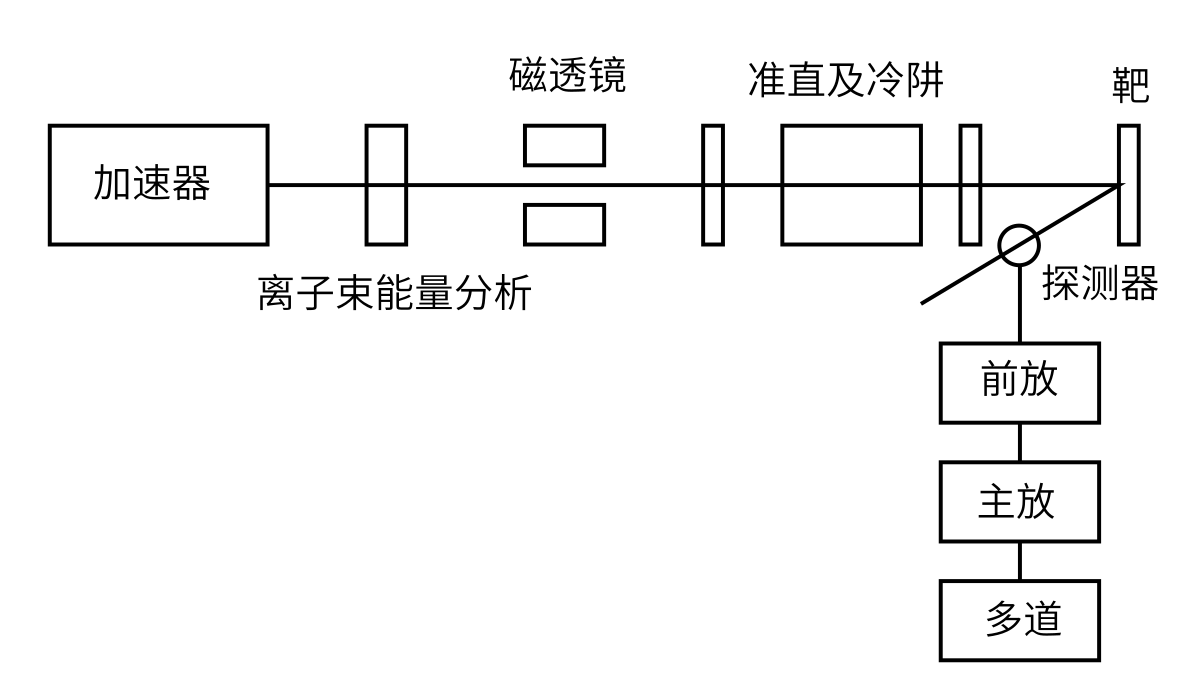
\includegraphics[width=0.45\textwidth]{shiyi.png}
\\
\xiaowu\song 图~1\begin{minipage}[t]{75mm} \quad 实验装置示意图。加速器产生的$\alpha$粒子经过处理后打靶并散射。后续探测器测量散射粒子的能谱。\\[-1mm]\wuhao
\end{minipage}
\end{center}

实验装置如图所示,加速器产生能量为2023KeV的$\alpha$粒子打入待测样品。探测器测量接收165度的散射粒子能谱。探测器选用的是金硅面垒探测器。因为$\alpha$粒子在空气中会很快的衰减,因而反应是在真空靶室中进行。

本实验中探测器的有效直径为3mm,探测器距离靶点8cm。

\section{实验过程和结果}
本实验使用SIMMRA软件来对收集到的散射能谱进行处理和分析。基本的思路是通过调节SIMMRA中的参数使得模拟能谱与实验能谱基本吻合,此时的参数应是靶的实际参数。

首先需要对系统进行检验和刻度。这时测量标样,在多道上得到相应的谱。因为标样由多个元素组成,因而分析可以得到系统的线性程度和刻度系数。先前同学得到的刻度系数如下: 

offset: 82.0KeV

Energy per channel: 3.713KeV/ch

在得到系统的刻度系数之后就可以测量待测样品了。该实验使用的待测样品是以Si作为基底,镀膜为ZnO掺杂EuO$_2$和Tm。测量得到的散射能谱图如下:

\begin{center}
   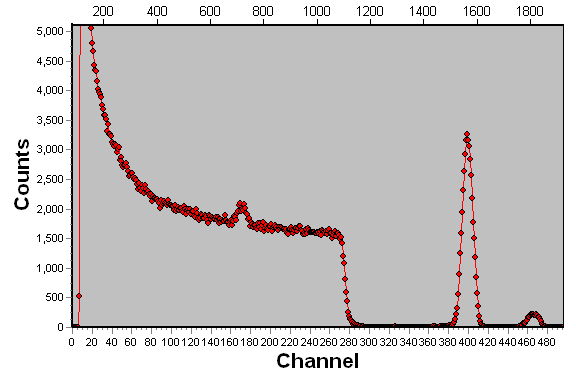
\includegraphics[width=0.45\textwidth]{1.png}
\\
\xiaowu\song 图~2\begin{minipage}[t]{75mm} \quad 样品散射能谱图。横坐标为道数,纵坐标为计数,顶部横坐标为散射粒子能量,单位为KeV。\\[-1mm]\wuhao
\end{minipage}
\end{center}

通过调整模拟参数,可以使得模拟的结果贴合实验的结果。模拟参数如下:
\begin{center}
   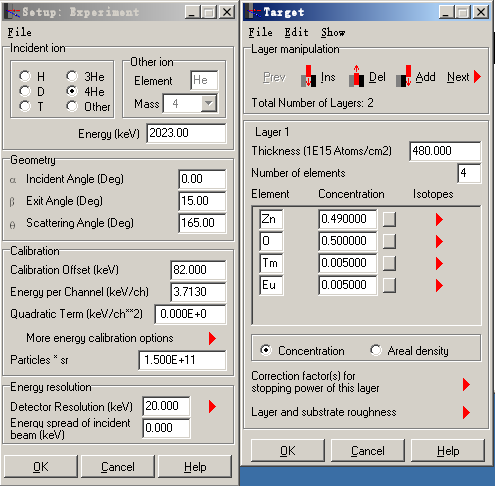
\includegraphics[width=0.45\textwidth]{2.png}
\\
\xiaowu\song 图~2\begin{minipage}[t]{75mm} \quad 模拟参数设定值。膜只有一层,成分比例为ZnO:EuO$_2$:Tm=100:1:1。衬底为Si基底。设置厚度为$8\times10^{21}Atoms/cm^2$\\[-1mm]\wuhao
\end{minipage}
\end{center}

如图所示,入射粒子为2023KeV的$\alpha$粒子,散射角度为165度,入射粒子数目乘立体角值为$1.50\times 10^{11}$。第一层膜为ZnO掺杂EuO$_2$,Tm,组分比为100:1:1,厚度为$4.8\times10^{17}Atoms/cm^2$。第二层为Si基底。模拟结果如下:
\begin{center}
   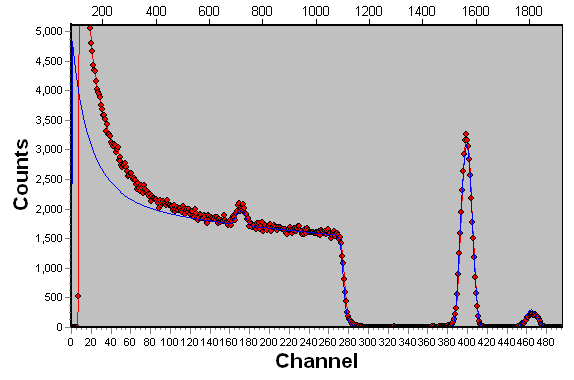
\includegraphics[width=0.45\textwidth]{3.png}
\\
\xiaowu\song 图~3\begin{minipage}[t]{75mm} \quad 模拟结果。蓝色线为模拟结果。\\[-1mm]\wuhao
\end{minipage}
\end{center}

如图所示,红色线为实验实测数据,蓝色线为模拟结果。一共有三个峰。在400道左右的应该是由于Zn产生的散射峰,而在470道左右的则可能是来源于Tm和Eu。因为两者质量数相近因而可能重叠不易区分。在180道左右有一个峰,这个峰应该是来自于O。从模拟结果来看,模拟和实际实验的相符性还是很高的。

图中在280道以下有一个坪,该坪应该是由Si产生的,Si基底的厚度非常厚,因而会因为电离等与电子相互作用的而损失能量,从而产生的就是一个坪,并在低道址附近有着很大的上升。

模拟得到的膜的厚度为$4.8\times10^{17}Atoms/cm^2$。由物质的组分可以得到平均的原子量为41.6。因为该材料主要又ZnO组成,因而可以将ZnO的密度认为为膜的密度。ZnO的密度为$5.61g/cm^3$,带入计算即可得到膜的厚度为:
\begin{equation}
	d=\frac{NA}{N_A\rho}=59.1nm
\end{equation}
其中$N_A$为阿伏加德罗常数,A为平均原子量,$\rho$为密度。

\section{总结和结论}
本实验使用背散射法测量样品的材料组分和厚度,得到样品的组分比例为:ZnO:EuO$_2$:Tm=100:1:1, 膜的厚度为59.1nm。

\section{致谢}
感谢娄建玲老师的细致地讲解以及为实验做出的准备。
\section{参考文献}

\noindent
[1] Peking Unviersity, Fudan University \ Nuclear Experment
\ Nuclear Publishing House, 1989: 269-278. (in Chinese)

\noindent
 (北京大学,复旦大学.\ 原子核实验\ 原子能出版社,\ 1989: 269-278.)
\end{multicols}

\newpage


\section*{附录:思考题}
1、根据表面散射出来的粒子能量E,我们可以确定材料的质量数目M。$K=\frac{E}{E_0}$,因而在因为探测器等因素造成测量粒子的能量有一定展宽为$\Delta E$时,$\Delta K=\frac{\Delta E}{E_0}$。 考虑K和M的关系,在大角度散射的情况下,有$K\approx(\frac{M-m}{M+m})^2$,因而有$\frac{dK}{dM}=\frac{4m(M-m)}{(M+m)^3}$。计算得到随着m从0逐渐增加到$(2-\sqrt(3))M$之间,该值逐渐增大。因而m越大,因E的展宽所造成的M
的展宽越小,所以选取质量数目较大的粒子可以增加质量分辨率。深度有$x=\Delta E/[S]$,因而S越大,深度分辨率越大,也就相当于使用更大质量的入射粒子。

2、入射能量太小的话无法进行深层的探测,而能量过大会使得散射截面变小,从而使分辨率下降,还有可能发生核反应等。因而能量不易过小或者过大。

3、由公式得到,当散射角为180度时有效散射截面最大,探测器探测到的散射粒子数目最多。但是因为其和入射束流重合而无法探测,因而在不影响束流的情况下散射角越大越好。

4、谱宽由能量分辨率,电子学噪声,加速器能量稳定性,真空度等等来决定。因而对于同一块靶,可能由于电子学噪声等造成谱宽不一致。

\clearpage
%\end{CJK*}
\end{document}



